%% IFBTcc Latex Template Version
%% 	based on a fork of : RiSE Latex Template
%%
%% IFBthesis latex template for thesis and dissertations
%% https://github.com/IFBmodels/tcc
%%
%% (c) 2017 Rafael de Campos Passos (rcpassos@ieee.org)
%%
%% This document was initially based on RiSE Latex template, from Yguaratã
%% Cerqueira Cavalcanti
%%
%% GENERAL INSTRUCTIONS
%%
%% We strongly recommend you to compile your documents using pdflatex command.
%% It is also recommend use the texlipse plugin for Eclipse to edit your documents.
%%
%% Options for \documentclass command:
%%         * Idiom
%%           pt   - Portguese (default)
%%           en   - English
%%
%%         * Text type
%%           bsc  - B.Sc. Thesis
%%           msc  - M.Sc. Thesis (default)
%%           qual - PHD qualification (not tested yet)
%%           prop - PHD proposal (not tested yet)
%%           phd  - PHD thesis
%%
%%         * Media
%%           scr  - to eletronic version (PDF) / see the users guide
%%
%%         * Pagination
%%           oneside - unique face press
%%           twoside - two faces press
%%
%%		   * Line spacing
%%           singlespacing  - the same as using \linespread{1}
%%           onehalfspacing - the same as using \linespread{1.3}
%%           doublespacing  - the same as using \linespread{1.6}
%%
%% Reference commands. Use the following commands to make references in your
%% text:
%%          \figref  -- for Figure reference
%%          \tabref  -- for Table reference
%%          \eqnref  -- for equation reference
%%          \chapref -- for chapter reference
%%          \secref  -- for section reference
%%          \appref  -- for appendix reference
%%          \axiref  -- for axiom reference
%%          \conjref -- for conjecture reference
%%          \defref  -- for definition reference
%%          \lemref  -- for lemma reference
%%          \theoref -- for theorem reference
%%          \corref  -- for corollary reference
%%          \propref -- for proprosition reference
%%          \pgref   -- for page reference
%%
%%          Example: See \chapref{chap:introduction}. It will produce
%%                   'See Chapter 1', in case of English language.
%%
%% Citation commands:
%%          \citet (from natbib) -- To cite a reference as part of the narrative
%%          \citep (from natbib) -- To cite a reference between parenthesis
%%          citationblock environment -- To produce direct citation blocks according to the ABNT

\documentclass[pt,twoside,onehalfspacing,bsc]{ifbclass/ifbclass}

  \usepackage{colortbl}
  \usepackage{color}
  \usepackage[table]{xcolor}
  \usepackage{microtype}
  \usepackage{bibentry}
  \usepackage{subfigure}
  \usepackage{multirow}
  \usepackage{rotating}
  \usepackage{booktabs}
  \usepackage{pdfpages}
  \usepackage{caption}
  \usepackage{lipsum}
  \usepackage{sectsty}
  \usepackage{tikz}
  \usepackage{amsmath}
  
  %% Set the language used in your code in the block above
  
  \captionsetup[table]{position=top,justification=centering,width=.85\textwidth,labelfont=bf,font=footnotesize}
  \captionsetup[lstlisting]{position=top,justification=centering,width=.85\textwidth,labelfont=bf,font=footnotesize}
  \captionsetup[figure]{position=bottom,justification=centering,width=.85\textwidth,labelfont=bf,font=footnotesize}
  
  %% Chapter and (Sub)Section fonts must be same size as text (12)
  \sectionfont{\fontsize{12}{15}\selectfont}
  \subsectionfont{\fontsize{12}{15}\selectfont}
  \subsubsectionfont{\fontsize{12}{15}\selectfont}
  
  %% Change the following pdf author attribute name to your name.
  \usepackage[linkcolor=black,
              citecolor=black,
              urlcolor=black,
              colorlinks,
              pdfpagelabels,
              pdftitle={IFB tcc Template (ABNT)},
              pdfauthor={ifb ctag team},
              breaklinks=true]{hyperref}
  
  \address{BRASÍLIA}
  
  \universitypt{Instituto Federal de Educação, Ciência e Tecnologia de Brasília, \textit{campus} Taguatinga,}
  \universityen{Federal Institute of Brasilia}
  
  \campus{Campus Taguatinga}
  
  \majorfieldpt{Bacharelado em Ciência da Computação}
  \majorfielden{Computer Science}
  
  \title{Comparação de ferramentas de sandboxing em sistemas GNU/Linux}
  
  \date{2023}
  
  \author{Ellian Aragão Dias, João Vitor Souza Rezende}
  \adviser{Daniel Saad}
  % \coadviser{Nome completo do co-orientador }
  
  % Macros (defines your own macros here, if needed)
  \def\x{\checkmark}
  %\let\lstlistoflistings\origlstoflistings
\begin{document}

\frontmatter

\frontpage

\presentationpage

\begin{fichacatalografica}
  \FakeFichaCatalografica % Comment this line when you have the correct file
  %     \includepdf{fig_ficha_catalografica.pdf} % Uncomment this
\end{fichacatalografica}

\banca

\begin{dedicatory}
  Obrigado a todos que acreditaram que eu poderia ser um belo garoto de programa
\end{dedicatory}

\acknowledgements
agradecimento

\begin{epigraph}[]{Márcio de Deus}
  When one finds a hard problem, the more complicated it is, the more one ought to work towards enlightening it's solution.
\end{epigraph}

\resumo
% Escreva seu resumo no arquivo resumo.tex
{\parindent0pt
  add intro

\begin{keywords}
add keyword
\end{keywords}
}

\abstract
% Write your abstract in a file called abstract.tex
{\parindent0pt
  The availability of various software ends up being something very common nowadays, even more with the wide adoption of broadband internet, because of this, not only the availability of authentic programs, we also have several malware that end up being coupled with some software and distributed as if they were the true version of these. Because of this the infection of computers with data hijacking and file encryption malware has become so common, the concern with security has been growing on the most diverse fronts. One solution is to make software execution secure, a concept also known as sandboxing, in which an application is executed in isolation from the system. This monograph makes a study of software that securely executes other programs, in order to analyze the base technologies applied to them, comparing and analyzing issues such as user friendly and performance, as well as proposing more appropriate use cases when applied within the Linux operating system.


\begin{keywords}
Software Security, Sandbox, Linux, Containers, Virtualization, Tools
\end{keywords}
}

% List of figures
% \listoffigures

% List of Codes
% \lstlistoflistings

% List of tables
% \listoftables

% List of acronyms
% Acronyms manual: http://linorg.usp.br/CTAN/macros/latex/contrib/acronym/acronym.pdf
% \listofacronyms
% \begin{acronym}[ACRONYM] 
% Change the word ACRONYM above to change the acronym column width.
% The column width is equals to the width of the word that you put.
% Read the manual about acronym package for more examples:
%   http://linorg.usp.br/CTAN/macros/latex/contrib/acronym/acronym.pdf
% parte que eu comecei a add
\acro{syscall}{chamada de sistema}
\acro{pid}[PID]{id de processo}
\end{acronym}

% Summary (tables of contents)
\tableofcontents

\mainmatter

\chapter{Introdução}
\label{chp:introduction}

justificar a existência do trabalho e porque ler

\begin{quotation}[]{Poul Anderson}
I have yet to see any problem, however complicated, which, when looked at in the
right way, did not become still more complicated.
\end{quotation}

Software maintenance starts as early as the first software artifacts are
delivered, and is characterized by its high cost and slow speed of
implementation~\citep{swebok2004}. It has been stated that it is the most
expensive activity of software development, taking up to 90\% of the total
costs~\citep{Eastwood1993,Erlikh2000}. However, despite of the high cost, it is
mandatory to ensure the success of the software project. \citet{Lehman1980}
argues, in his \emph{Continuing Change} law of software evolution, that the
modification of software is a fact of life for software systems if they are
intended to remain useful. \citet{Bennett2000} reinforced such an argument for
the specific case of useful and successful software, where almost all of them
have a common practice of stimulating user-generated \ac{cr}. Actually, software
maintenance is driven by \acp{cr} reported by many stakeholders, such as
developers, testers, team leaders, managers, and clients.

In this context, the \ac{cr} repositories play an important role in the
maintenance and evolution process, being actually a focal point of communication
and coordination for software projects~\citep{Bertram2010}. Through a \ac{cr}
repository, the developers manage and coordinate the corrections and new
features to be implemented in the software under development or maintenance.
Moreover, the data stored in such repositories are a valuable source of
information about the project, which can be used to assist in cost estimation,
impact analysis, traceability, planning, expertise discovery, and software
understanding \citep{CavalcantiSQJ2011}. Examples of these repositories are
Mantis~\citep{Mantis}, Bugzilla~\citep{Bugzilla}, and Trac~\citep{Trac}.

Briefly, a \ac{cr} describes a defect to be fixed, an adaptive or perfective
change, or a new functionality to be implemented in a software
system~\citep{CavalcantiSQJ2011}. Each \ac{cr} stores a variety of fields of
free text and custom fields defined according to the necessity of each project.
In Trac, for example, it has fields for summary and detailed description of a
\ac{cr}. In the same \ac{cr}, it can be also recorded information about software
version, dependencies with other \acp{cr} (such as \acp{cr} that are blocked,
similar, or duplicate), the person who will be assigned to the \ac{cr}, among
other relevant information. Moreover, during the life cycle of a \ac{cr},
different kinds of discussion take place through the comments that are inserted
in it, such as fixing alternatives, workarounds, and architectural
decisions~\citep{Bertram2010}.

\section[Motivation  (Why to Automate CR Assignment?)]{Motivation (Why to
Automate \ac{cr} Assignment?)}

Despite \ac{cr} repositories claimed benefits to software maintenance and
evolution, handling \acp{cr} is not cost-free. For example, when new \acp{cr}
are reported they must be assigned to developers which have adequate expertise
to address the request~\citep{Aljarah2011,Hosseini2012,Kagdi2012}. Finding the
appropriate developer is crucial for obtaining the lowest, economically
feasible, fixing time~\citep{Lucca2002}. Nevertheless, assigning \acp{cr} to
developers is a labor-intensive and time consuming
task~\citep{Anvik2006,Jeong2009}. Indeed, depending on the project being
developed, the amount of \acp{cr} that are reported and need to be assigned can
vary from dozens to hundreds per day~\citep{CavalcantiSQJ2011}.

\figref{fig:assignment-schema} shows the activity of assigning \acp{cr}.
At the top-left corner of the figure, there are the \acp{cr} which have been
reported to the software project. At the bottom-left corner, there is a set of
developers which could be assigned to those \acp{cr}. Then, at the center, the
assignment of \acp{cr} is performed; the \acp{cr} and developers must be
matched, and each developer should fix one or more \acp{cr}. Commonly, the
matching is performed aiming at the shortest time and the highest quality for
the \ac{cr} fixing activities.

\begin{figure}[htp]
\centering
  \caption[\ac{cr} assignment.]{\ac{cr} assignment. The router, which may be the
  \acs{ccb}, project leaders, or managers, must match \acp{cr} and developers in
  order to obtain the shortest fixing and highest quality.}
  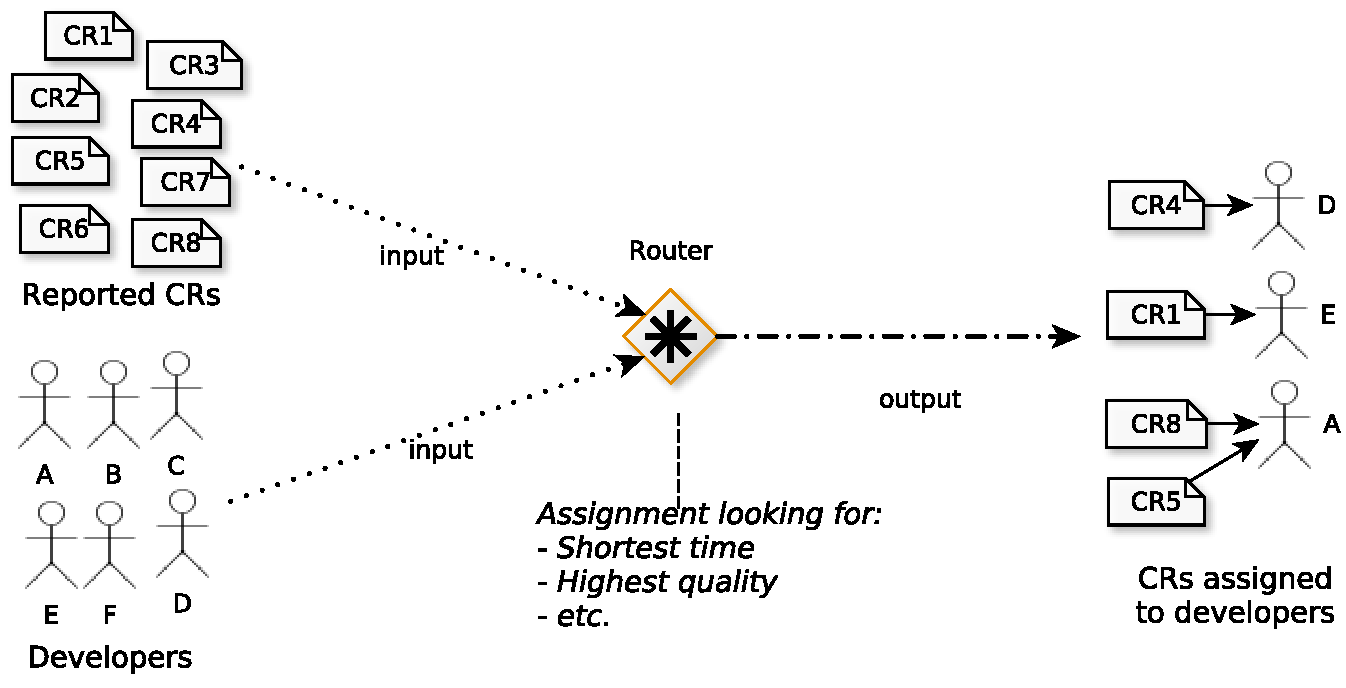
\includegraphics[width=\columnwidth]{images/assignment-schema.pdf}
  \footnotesize{Source: Made by the author.}
  \label{fig:assignment-schema}
\end{figure}


Nevertheless, by increasing the amount of reported \acp{cr} or the size of the
development team, it is visible that the router becomes overloaded and the
\ac{cr} assignment becomes an intensive, error prone activity. It was confirmed
by \citet{Jeong2009}, which identified that 37\%-44\% of the \acp{cr} in Mozilla
and Eclipse projects did not reach the right developer in the first assignment.
These \acp{cr}, in turn, had their fixing time delayed because they needed to be
reassigned one or more times. Furthermore, if the \acp{cr} are not fixed by the
appropriate developers, there is also the chance of introducing new defects
during the \acp{cr} fixing.

In this context, we believe that it is necessary to develop methods and tools to
automate the assignment of \acp{cr} and ensure that the \acp{cr} are being
assigned to the appropriate developers. With these methods and tools, we could
reduce the time needed to perform the assignments and, given that the
appropriate developers are actually being selected, the quality and time for the
\ac{cr} fixing are also improved.

\section{Problem Statement}
\label{sec:intro-problem-statement}

As previously mentioned, software maintenance has been considered as the most
costly aspect of software development~\citep{swebok2004}. There is a myriad of
reasons for this situation. One of them is the many changes that are required
after software delivery due to poor documented and misunderstood requirements,
or simply because \emph{``the clients do not know what they
want''}~\citep{Brooks1995}.

Another reason is the fact that a set of development activities must be
inevitably performed in order to implement a change. For instance, for each
change to be implemented it is necessary to comprehend the existing software
artifacts, modify the software's source code to implement the change, perform
tests and verification, and deliver the new version of the software.
Additionally, very often, the implementation of the change ends up by
introducing new defects in the software.

A third reason is the management aspects of software maintenance. It is
necessary to keep track of all these changes that are performed, generally
considering different versions of the software and customers.


\begin{enumerate}
  \item Firstly, the approaches available in the literature were designed to
  perform autonomously. That is, the software analysts do not have the control
  of the approach; they cannot modify the approach's behavior. Without
  such control, in turn, the approach cannot be properly calibrated. As a
  consequence, if the approach's performance is not satisfactory, it is simply
  discarded.
  \item Secondly, the reported values for accuracy of these approaches are
  still low. With low accuracy, the previous reason takes place. That is, as the
  approaches perform with low accuracy, and the software analysts do not have
  control over them, the approaches are simply discarded.
  \item Finally, the third reason concerns the lack of contextual information in
  those approaches. As is well known, software development companies are
  dynamic: developers move from projects; developers are hired/fired;
  developers enter in vacation or take a day off; and developers have different
  experiences. This dynamic influences the assignment of \acp{cr}. Thus,
  contextual information is a necessity in automated approaches.
\end{enumerate}

Based on this context, the main research question investigated by this thesis is:

\begin{description}
  \item[Research question] \emph{Is it possible to develop a new approach for
  automated \ac{cr} assignment with satisfactory accuracy, leveraging
  contextual information, and designed in order to put the software analysts in
  control of such approach?}
\end{description}

With the objective to answer this question, it is necessary to understand
current approaches available in the literature, choose the correct technologies
that could support dynamic environments and, mainly, understand the necessities
of software analysts regarding a new approach for automated \ac{cr} assignment.
Thus, the goal of the work described in this thesis can be stated as:

\begin{description}
  \item[Research objective] \emph{This work proposes an automated approach for
  \ac{cr} assignment which uses \ac{ir} models, expert systems, and
  context-aware information in order to select the appropriate developers. The
  approach is supported by the state-of-the-art in the management of \acp{cr} as
  well as by the understanding of the aspects concerning the \ac{cr} assignment
  activity itself.}
\end{description}


\section{Research Methodology}

This research design of this thesis is based on a multimethod
approach~\citep{Hesse-Biber2010}. Such approach combines two or more
quantitative (or qualitative) methods in a single study, such as a survey and an
experiment~\citep{Hesse-Biber2010}. Multimethod must not be confused with mixed
method. In this last, methods for both qualitative and quantitative types of
research are applied in a single study. On the other hand, multimethod studies
combine different methods for a single research type.

When applying a multimethod approach, the triangulation is used to consolidate
the results from the different methods, considering, however, that the same
research question(s) was/were investigated in these methods. As a consequence,
the triangulation of methods enhances the conclusions and completeness of the
study, bringing more credibility to the research
findings~\citep{Hesse-Biber2010}. \figref{fig:research-methodology-thesis} shows
the multimethod research design applied in this thesis.

\begin{figure}[h]
\centering
  \caption[Research methodology.]{The research methodology applied for this
  thesis.}
  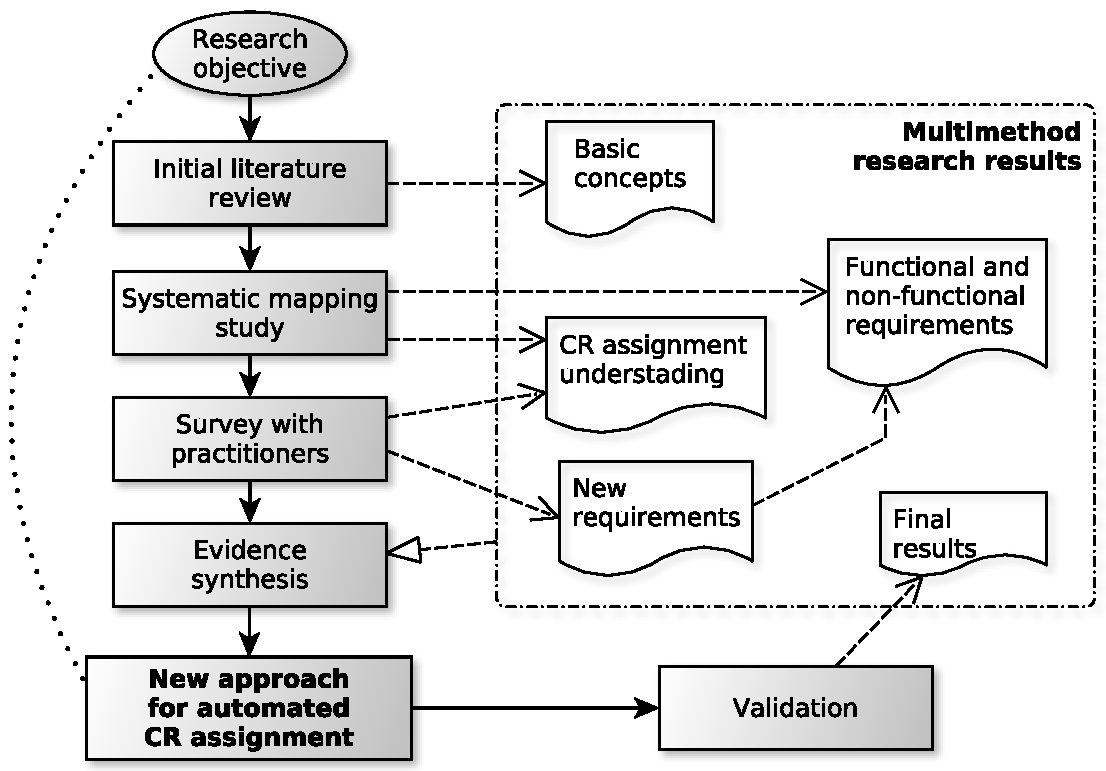
\includegraphics[width=\columnwidth]{images/research-methodology-thesis.pdf}
  \footnotesize{Source: Made by the author.}
  \label{fig:research-methodology-thesis}
\end{figure}

The design started by stating the research objective, which we defined in
\secref{sec:intro-problem-statement}, and performing the initial literature
review. This last provided the basic concepts and understanding of the area.
Then, a systematic mapping study and a questionnaire-based survey were
conducted. These two gathered detailed information on our research topic.
Indeed, both of them were used to understand the key aspects of \ac{cr}
assignment and identify the set of requirements to automate the assignments. In
the evidence synthesis step, these results were detailed and organized in order
to formulate the approach to automate \ac{cr} assignments, which was constructed
in the next step. Finally, the research design states the validation of the
proposed approach.

\section{Out of Scope}

As the proposed approach is part of a broader context, a set of related aspects
will be left out of its scope. Thus, the following topics are not directly
addressed in this thesis:

\begin{enumerate}
  \item \textbf{Tools for \ac{cr} management.} We are addressing
  a specific aspect of \ac{cr} management, which is the \ac{cr} assignment
  activity. Thus, it is out of scope of this thesis to provide a
  complete solution for \ac{cr} management. Instead, we are planning to
  implement standalone software which will be able to integrate with the
  most well known tools for \ac{cr} management, such as Mantis, Bugzilla, and
  Trac, providing a service to leverage the automation of \ac{cr}
  assignments.

  \item \textbf{Software maintenance process.} Software maintenance involves
  a set of activities aiming at implementing modifications in some software
  project. These activities must be coordinated through a process so that the
  maintenance can be successful. In Chapter 2, we discuss some of
  these processes. However, in this thesis, we are not concerned with the
  maintenance process itself. Actually, it should be transparent in our approach
  to automate \ac{cr} assignment. Thus, it is out of scope of this
  thesis to provide any process assessment for software maintenance beyond the
  activity of \ac{cr} assignment.

  \item \textbf{\ac{ir} models.} Many models for \ac{ir} have been proposed for
  different objectives, including the \ac{cr} assignment itself. However, due to
  the broad availability of these models, it is out of scope of this thesis to
  develop a new one. Instead, the \ac{ir} models with better performance,
  identified through the systematic mapping study, were chose to be
  integrated in our approach;

  \item \textbf{Rule-based expert systems.} Similar to \ac{ir} models,
  rule-based expert systems have a long history of development. Thus, our
  approach does not intend to develop a whole new system with this purpose.
  Actually, we integrated in our approach the
  Drools\footnote{\url{http://www.jboss.org/drools/}} expert system, which is a
  mature tool that can be easily manipulated;

  \item \textbf{Mathematical formulations on NP-Complete problems.} We
  understand that the problem of assigning \acp{cr} to software developers is in
  the broad category of \emph{assignment problems}, which is well known to be
  NP-Complete. Thus, could be formulated as such. However, the mathematical
  formulations of the \ac{cr} assignment problem is out of scope of this thesis.
  As well as finding an optimal solution on the context of NP-Complete problems
  is also out of scope. The main reason for this is the human factors and
  context variables that are involved in the assignment of \acp{cr}, which
  make this problem hard to be computable. A mathematical formulation of the
  \ac{cr} assignment problem is provided by~\citet{Rahman2009}.
\end{enumerate}

\begin{enumerate}
  \item An overview of the software maintenance concepts and processes, with
  emphasis on the importance of \ac{cr} management aspects;
  \item A survey performed with practitioners from a large organization, in
  order to understand the aspects of the \ac{cr} assignment
  activity. Published in the \emph{17$^{th}$ International Conference on Evaluation
  and Assessment in Software Engineering (EASE'2013)}~\citep{CavalcantiEASE2013};
  \item A replication of the previous survey in two more organizations;
  \item A systematic mapping study performed to understand the challenges and
  opportunities of \ac{cr} management, as well as to identify research gaps and
  the road ahead. Accepted for publication in the
  \emph{Journal of Software: Evolution and Process}~\citep{CavalcantiJSEP2013};
  \item The definition of the functional and non-functional requirements that
  are required to effectively automate \ac{cr} assignment, which takes as input
  the systematic mapping study and the survey;
  \item The definition of an approach that satisfies the
  identified requirements to automate the \ac{cr} assignment activity;
  \item The realization of the proposed approach's architecture, in which we
  described the methods and techniques used for the implementation, as well as the
  components that have to be built and the third party components that should be
  assembled together in order to provide a service for automated \ac{cr}
  assignment; and
  \item The evaluation of the proposed approach, performed as an offline
  experiment simulating a real context.
\end{enumerate}
\chapter{Referencial teórico}

Como base do conteúdo a ser referenciado dentro deste trabalho, existem diversas tecnologias e conceitos que são de fundamental importância a compreensão de modo que seja entendido desde os comparativos a de fato como as ferramentas a serem tratadas funcionam e interagem com o kernel Linux. Diante disto, temos a seguir alguns conceitos a serem expostos de modo a clarificar a sua importância e a base das ferramentas a serem tratadas, nestas temos namespaces e cgroups como os conceitos mais importantes e utilizados diante de todos os softwares a serem comentados posteriormente.

\section{Namespace}
A tecnologia consiste em fazer o isolamento dos recursos a serem utilizados por determinado software que esteja rodando. Deste modo o namespace é uma camada de interação que se encontra entre a sua execução propriamente dita e sua interação com kernel, tal como um proxy \cite{kernelscheepers}.

Como comentado, esta camada que encontra-se entre o processo e o kernel, atua quando determinado software executa uma syscall (chamada de sistema) e as estruturas do processo, possuem os dados de determinado namespace, este que por sua vez delimita que recursos estão disponíveis para serem utilizados.

Desta forma cria-se uma virtualização dos recursos que são disponíveis e quais são eles, uma vez que a resposta para o software a ser executada é dada pelas configurações daquele namespace sob o qual a aplicação roda. Sendo esta a base para criação de containers, dos quais trata-se de um processo o qual roda de maneira isolada sob um sistema operacional.

Por fim, uma vez compreendida sua função, é necessário a compreensão de quais tipos de namespaces estão disponíveis uma vez que utilize-se o kernel posterior 5.6 do linux.

\section{Cgroups}
O controle de grupos, também chamado de cgroups, é a ferramenta para controle de uso do recurso, sendo esses de alguns tipos diferentes, mas em seu cerne trata-se de controle de quantidade de uso deste, ou seja quanto tempo ou banda de utilização de determinado recurso estaria liberado para um determinado processo do qual se encontra sob aquele cgroup.

Compreendido que se trata do uso de recurso, aqueles que estão sob controle de determinado grupo, pode-se limitar o uso da CPU e utilização de blocos de I/O (entrada e saída de dados). Deste modo pode-se determinar quanto tempo de processamento está disponível e/ou quantos bytes estão disponíveis na entrada e saída do processo, seja ela utilização de rede (internet), escrita e leitura de arquivos, etc...

\section{Containers}

\section{Virtualização}

\chapter{Ferramentas de Sandboxing}

\section{AppArmor}
O AppArmor é um sistema de controle de acesso obrigatório (MAC - Mandatory Access Control) que oferece recursos de segurança adicionais ao sistema operacional Linux. Ele permite aos administradores do sistema criar políticas de segurança personalizadas para controlar o acesso de processos e aplicativos a recursos do sistema, como arquivos, diretórios, portas de rede e outros.

O objetivo do AppArmor é restringir o acesso a esses recursos, limitando as ações que um processo pode realizar, a fim de evitar a execução de código malicioso ou não autorizado. Ao utilizar o AppArmor, os administradores podem criar perfis de segurança que definem as permissões e restrições para cada aplicativo em execução no sistema.

\subsection{Configuração}
A configuração do AppArmor envolve a definição de perfis de segurança para cada aplicativo. Esses perfis especificam quais recursos do sistema o aplicativo pode acessar e quais ações ele pode realizar. Essa configuração pode ser feita por meio de arquivos de perfil ou usando ferramentas de linha de comando fornecidas pelo AppArmor.

Embora o AppArmor seja uma ferramenta poderosa para aumentar a segurança do sistema, é importante notar que ele não é uma solução completa. É recomendado que os administradores de sistema adotem uma abordagem em camadas para a segurança, combinando o uso do AppArmor com outras medidas de proteção, como atualizações regulares de segurança e práticas de segurança recomendadas.

\subsection{Integração com linux}

Uma das principais características do AppArmor é sua integração com o kernel do Linux. Ele aproveita os recursos de segurança fornecidos pelo kernel, como namespaces e cgroups, para isolar os processos em seus próprios ambientes protegidos. Essa abordagem garante um bom desempenho e uma pegada de recursos mínima.

\subsection{gerenciando os perfis}

O AppArmor, no Linux, oferece um sistema flexível de gerenciamento de perfis que permite aos administradores do sistema controlar as políticas de segurança de forma granular. Os perfis são arquivos de configuração que definem as permissões e restrições de acesso para cada aplicativo ou processo em execução no sistema.

No AppArmor, o gerenciamento de perfis envolve três etapas principais: criação, configuração e aplicação dos perfis.

A criação de um perfil é a etapa em que um administrador define as permissões e restrições desejadas para um aplicativo específico. O perfil é geralmente escrito em uma linguagem de configuração, como o AppArmor Profile Language (AAPL) ou usando uma abordagem baseada em aprendizado de perfil, onde o AppArmor registra as ações do aplicativo durante uma sessão de treinamento e cria um perfil com base nesses registros.

A configuração de um perfil envolve especificar as permissões necessárias para que o aplicativo funcione corretamente. Isso pode incluir permissões para acessar arquivos, diretórios, dispositivos, sockets de rede e outras entidades do sistema. As restrições também podem ser aplicadas, limitando as ações que o aplicativo pode executar, como impedir o acesso a certas partes do sistema de arquivos ou restringir o uso de recursos de rede.

Uma vez que o perfil tenha sido criado e configurado, ele pode ser aplicado ao aplicativo ou processo específico. O AppArmor suporta diferentes métodos de aplicação de perfil, como associar o perfil a um binário específico, atribuí-lo a um namespace ou usar as ferramentas de linha de comando do AppArmor para aplicar o perfil dinamicamente.

Além disso, o AppArmor suporta o conceito de herança de perfil, onde é possível criar perfis base e perfis dependentes. Os perfis dependentes herdam as permissões e restrições dos perfis base, permitindo a criação de hierarquias de perfis que facilitam o gerenciamento de políticas de segurança em larga escala \cite{debian-handbook}.

É importante destacar que o AppArmor fornece recursos avançados de auditoria e registro de eventos. Os logs do AppArmor registram violações de segurança, permitindo aos administradores analisar e solucionar problemas relacionados à configuração de perfil e detectar possíveis ameaças. 

\subsection{exemplos}
 Considere um servidor web que executa um aplicativo da web. Podemos criar um perfil de segurança específico para esse aplicativo, limitando seu acesso apenas aos arquivos e diretórios necessários para operar corretamente. Isso restringe o impacto de um possível ataque, limitando as ações que um invasor pode realizar dentro do ambiente restrito do aplicativo.

Outro exemplo é o uso do AppArmor em ambientes de desktop, onde aplicativos como navegadores da web são comumente usados. Ao aplicar perfis de segurança a esses aplicativos, podemos restringir seu acesso a informações confidenciais, como arquivos pessoais do usuário, protegendo assim a privacidade e evitando a exfiltração de dados.
\section{Bubblewrap}

 Ferramenta de sandboxing amplamente utilizada no ecossistema Linux, como no seu derivado flatpak, Ele fornece um ambiente seguro e isolado para a execução de aplicativos, permitindo que eles operem com um nível mínimo de privilégios e restrições de acesso. O Bubblewrap baseia-se em recursos avançados do kernel do Linux, como namespaces e cgroups, para oferecer isolamento de processos e limitação de acessos \cite{bubblewrap-github, bubblewrap-archlinux}.

\paragraph*{Isolamento de processos}\mbox{}\\
Ele cria um ambiente separado para a execução de aplicativos, isolando-os uns dos outros e do sistema operacional hospedeiro. Cada aplicativo em execução dentro do sandbox do Bubblewrap é encapsulado em seu próprio conjunto de namespaces, como de rede, sistema de arquivos e hostname. Isso impede que os processos dentro do sandbox afetem outros processos ou acessem recursos do sistema não autorizados \cite{linux-containers-virtualization}.

\paragraph*{Limitação de acesso}\mbox{}\\
A limitação de acesso é outra característica fundamental do Bubblewrap. Ele permite que os administradores configurem políticas de segurança detalhadas para restringir o acesso dos aplicativos a recursos específicos do sistema. Por exemplo, é possível limitar o acesso a arquivos, diretórios, dispositivos, sockets de rede e outros recursos essenciais. Essa abordagem granular ajuda a evitar que aplicativos comprometidos acessem dados sensíveis ou executem operações indesejadas \cite{linux-security-redhat, bubblewrap-archlinux}.

 Sendo amplamente utilizado em diferentes cenários, é uma parte essencial do ecossistema de empacotamento de aplicativos Flatpak, permitindo que os aplicativos sejam executados em um ambiente seguro e isolado. Ele também pode ser usado para criar ambientes de teste isolados, facilitando a execução de aplicativos sem risco de impacto no sistema operacional hospedeiro 
 \cite{bubblewrap-github, bubblewrap-archlinux}.

\paragraph*{Exemplo}\mbox{}\\
Um exemplo prático do uso é a execução de um navegador da web em um sandbox. Ao executar o navegador dentro de um sandbox do Bubblewrap, é possível limitar seu acesso ao sistema de arquivos, restringir permissões de rede e impedir que ele acesse informações confidenciais. Isso aumenta a segurança, reduzindo a superfície de ataque em caso de exploração de vulnerabilidades do navegador.
\section{Capsicum}

Ferramenta de segurança e sandboxing desenvolvida para o sistema operacional FreeBSD, embora também tenha sido portado para outros sistemas, como o Linux. Ele oferece recursos avançados de isolamento de processos e restrição de acesso, com foco na minimização de vulnerabilidades e na proteção de aplicativos contra ataques cibernéticos.

As principais características do Capsicum é a implementação do modelo de sandbox baseado em recursos, que permite aos desenvolvedores restringir o acesso de aplicativos somente aos recursos necessários para sua execução. Isso é alcançado através do conceito de "capabilidades" (capabilities), que são permissões granulares que um processo pode ter para acessar recursos do sistema. O Capsicum permite que os desenvolvedores reduzam essas capabilidades para um processo, limitando assim seu poder e evitando a exploração de vulnerabilidades.

\subsection{Separação de contexto}

Tendo a separação de contexto, que é alcançada através do uso de descritores de arquivos e recursos encapsulados chamados "sandbox". Essa separação de contexto permite que um processo tenha acesso somente a um subconjunto específico de recursos, limitando sua capacidade de interagir com outros processos ou modificar recursos não autorizados.

Suporta o uso de descritores de arquivos com limitação de escopo, onde um processo pode restringir o acesso a um conjunto específico de descritores de arquivos. Isso ajuda a prevenir a escalada de privilégios, impedindo que um processo acesse outros arquivos ou recursos além dos permitidos.

\subsection{exemplos}

Uma aplicação prática do Capsicum é a proteção de aplicativos com vários componentes que precisam interagir entre si, mas sem expor todos os recursos do sistema a cada componente. Com o Capsicum, é possível definir capabilidades específicas para cada componente, limitando assim seu acesso a recursos específicos e reduzindo o impacto caso algum componente seja comprometido.
\section{Docker}

O Docker é uma plataforma de software que permite aos desenvolvedores criar, implantar e executar aplicativos em contêineres. O principal objetivo do Docker é facilitar a implantação e o gerenciamento de aplicativos, fornecendo um ambiente consistente e isolado para sua execução \cite{docker-docs}.

\paragraph*{Containers}\mbox{}\\
 Um container é uma unidade de software que encapsula um aplicativo e todas as suas dependências, incluindo bibliotecas, frameworks e arquivos de configuração. Diferentemente das máquinas virtuais tradicionais, os contêineres compartilham o mesmo kernel do sistema operacional hospedeiro, o que os torna mais leves e eficientes \cite{linux-containers-virtualization,docker-docs}.

\paragraph*{Portabilidade}\mbox{}\\
A portabilidade é outra característica-chave do Docker. Os contêineres Docker são independentes da plataforma e podem ser executados em qualquer ambiente que tenha o Docker instalado, seja localmente em um computador de desenvolvimento ou em um ambiente de nuvem como o AWS, Google Cloud Platform ou Microsoft Azure. Isso facilita a implantação consistente de aplicativos em diferentes ambientes, eliminando problemas de compatibilidade \cite{docker-book,docker-aws}.

\paragraph*{Gerenciamento de imagens}\mbox{}\\

Uma imagem Docker é uma representação estática de um contêiner, contendo todas as dependências e configurações necessárias. As imagens são criadas usando arquivos de configuração chamados Dockerfiles, que descrevem os passos para configurar o ambiente do contêiner. Isso torna a criação e o compartilhamento de aplicativos e suas dependências mais fáceis e reproduzíveis.

\paragraph*{Escabilidade}\mbox{}\\

Com o Docker Swarm ou o Kubernetes, é possível implantar aplicativos em clusters de máquinas, permitindo a execução de várias réplicas de um aplicativo para lidar com altas cargas de tráfego. Essa capacidade de escalabilidade horizontal ajuda a garantir a disponibilidade e o desempenho de aplicativos em ambientes de produção \cite{docker-docs,docker-book,docker-aws}.

Permitindo a criação de redes virtuais isoladas para os contêineres. Isso possibilita a comunicação segura entre contêineres, bem como a exposição controlada de portas para comunicação com o mundo externo.
\section{Firejail}

Uma ferramenta de sandboxing que oferece um ambiente seguro para a execução de aplicativos Linux. Sua principal finalidade é isolar processos e restringir o acesso a recursos do sistema, fornecendo uma camada adicional de segurança.

Uma das características mais importantes do Firejail é o uso de namespaces do kernel do Linux para criar um ambiente isolado para o aplicativo. Ele utiliza namespaces como PID, rede, sistema de arquivos e usuários para separar o aplicativo em execução do restante do sistema. Isso evita que o aplicativo acesse ou modifique recursos sensíveis do sistema, reduzindo o risco de ataques \cite{firejail-archwiki}.

Ele também fornece controle granular sobre as permissões de acesso do aplicativo. Por meio de perfis de segurança, podendo especificar quais recursos o aplicativo pode acessar e quais ações ele pode realizar. Isso inclui restrições em acesso a arquivos, diretórios, sockets de rede, dispositivos e muito mais. Com essas permissões definidas, o Firejail garante que o aplicativo funcione somente dentro dos limites especificados.

\paragraph*{Segurança}\mbox{}\\
 Como a proteção contra a fuga de informações através de áreas de transferência (clipboard), prevenção de captura de tela e restringir o acesso a recursos de servidores de exibição gráfica, tais como Xorg (X11) e Wayland. Essas medidas extras ajudam a proteger informações sensíveis e impedir que aplicativos maliciosos realizem ações indesejadas.
 
Ele pode ser executado diretamente na linha de comando, envolvendo o comando do aplicativo que se deseja executar em sandbox. Também é possível criar perfis de segurança personalizados que podem ser compartilhados e reutilizados nas aplicações.

\paragraph*{}\mbox{Utilização}\\
O Firejail é frequentemente utilizado para a execução de navegadores da web, clientes de email e outros aplicativos suscetíveis a ataques. Com o Firejail, é possível mitigar o impacto de vulnerabilidades do aplicativo, limitando sua capacidade de acessar recursos do sistema e restringindo sua interação com outros processos em execução.
\section{LXC}
\section{OpenVZ}

O OpenVZ é uma plataforma de virtualização de sistema operacional que permite a criação de ambientes virtuais isolados, chamados de "contêineres", em um único servidor físico. Essa tecnologia oferece uma abordagem eficiente e escalável para virtualização, permitindo a execução de múltiplos sistemas operacionais em um único host.

\subsection{Eficiência e baixa sobrecarga}
 Ao contrário das soluções de virtualização completa, onde cada máquina virtual (VM) executa seu próprio kernel do sistema operacional, o OpenVZ compartilha um único kernel entre os contêineres. Essa abordagem compartilhada resulta em um melhor desempenho e eficiência, com menor utilização de recursos, uma vez que os contêineres não precisam carregar um sistema operacional completo.

\subsection{Isolamento avançado}
Cada contêiner é completamente isolado, com seu próprio sistema de arquivos, processos, rede e recursos alocados, proporcionando um ambiente seguro e protegido. O isolamento impede que os contêineres afetem uns aos outros e permite que cada contêiner opere independentemente, como se fosse uma instância virtualizada separada.

Além disso, o OpenVZ fornece recursos avançados de gerenciamento de recursos. Os recursos, como CPU, memória e espaço em disco, podem ser alocados e limitados de forma granular para cada contêiner. Isso permite um controle preciso e equilibrado do uso de recursos, garantindo que nenhum contêiner monopolize os recursos do sistema.

\subsection{Escalabilidade}
Sendo possível criar e gerenciar facilmente um grande número de contêineres em um único servidor físico, essa capacidade de dimensionamento horizontal permite que os administradores maximizem a utilização dos recursos e implantem aplicativos em escala, atendendo a demandas crescentes.

\subsection{Gerenciamento e monitoramento abrangentes}
 Criação trazendo  facilitação para uma administração dos contêineres, existindo interfaces de linha de comando e interfaces gráficas disponíveis para gerenciar, monitorar e fazer ajustes nos contêineres.
\section{Podman}

O Podman é uma ferramenta de gerenciamento de contêineres de código aberto que permite a criação, execução e gerenciamento de contêineres no ecossistema Linux. Ele é projetado para ser uma alternativa ao Docker, fornecendo recursos semelhantes enquanto se concentra em segurança, simplicidade e compatibilidade com o padrão Open Container Initiative (OCI).


\subsection{Daemon}
Ao contrário do Docker, que usa um daemon em execução em segundo plano, o Podman utiliza uma arquitetura sem daemon, executando os contêineres diretamente como processos no espaço de usuário. Isso resulta em um ambiente de execução mais seguro, eliminando a necessidade de um processo em execução em segundo plano com privilégios elevados.

\subsection{Isolamento robusto}
O Podman também oferece isolamento robusto de contêineres por meio do uso de namespaces e cgroups do kernel Linux. Ele permite a criação de contêineres isolados que possuem seu próprio ambiente de sistema de arquivos, processos, rede e outros recursos. Isso garante que os contêineres executados pelo Podman operem de forma independente, sem afetar uns aos outros ou o sistema operacional hospedeiro.

\subsection{Padrão OCI}
Significa que os contêineres criados com o Podman são compatíveis com outros sistemas de execução de contêineres que aderem ao mesmo padrão, como o Docker. Isso permite que os usuários compartilhem e distribuam contêineres facilmente entre diferentes ambientes e ferramentas compatíveis com OCI.

O Podman fornece um conjunto abrangente de comandos de linha de comando que permitem a criação, execução e gerenciamento de contêineres. Ele suporta recursos avançados, como criação de redes virtuais, montagem de volumes, configuração de variáveis de ambiente e execução de comandos dentro de contêineres em execução. Isso oferece flexibilidade e controle aos usuários para personalizar e ajustar seus contêineres de acordo com suas necessidades.

\subsection{Segurança}
 Podman oferece suporte a recursos de segurança, como o uso de SELinux para aplicar políticas de segurança e restrições adicionais nos contêineres. Ele também oferece recursos de gerenciamento de imagens e compartilhamento de contêineres através de registros e repositórios.
\section{Seccomp}

O Seccomp é uma ferramenta de segurança avançada disponível no kernel do Linux que permite restringir as chamadas de sistema (system calls) disponíveis para um processo em execução. Sua principal finalidade é aumentar a segurança do sistema, limitando as possíveis vias de ataque que um aplicativo pode explorar.

Uma das principais características do Seccomp é a capacidade de filtrar as chamadas de sistema permitidas para um processo. Ele permite que os administradores ou desenvolvedores definam uma política de segurança, especificando quais chamadas de sistema são permitidas e quais devem ser bloqueadas. Isso reduz a superfície de ataque do aplicativo, pois impede que ele faça chamadas de sistema potencialmente perigosas ou desnecessárias.

O Seccomp funciona usando um filtro BPF (Berkeley Packet Filter), que é um mecanismo de filtragem de pacotes flexível e eficiente. O filtro BPF é usado para especificar as regras do Seccomp, determinando quais chamadas de sistema são permitidas ou bloqueadas com base em critérios definidos. Essas regras podem ser aplicadas a um processo específico ou a um grupo de processos.

Outra característica importante do Seccomp é sua capacidade de fornecer um ambiente de execução seguro para aplicativos não confiáveis ou suspeitos. Por exemplo, em ambientes de contêineres, o Seccomp pode ser usado para restringir as chamadas de sistema disponíveis para um contêiner, garantindo que ele não acesse recursos ou execute operações não autorizadas. Isso ajuda a mitigar o impacto de possíveis ataques e limita as ações que um aplicativo malicioso pode realizar.

Além disso, o Seccomp é altamente flexível e suporta diferentes níveis de filtragem. Pode ser usado tanto em modo de auditoria, apenas registrando as chamadas de sistema que seriam bloqueadas, quanto em modo de execução real, bloqueando efetivamente as chamadas de sistema não permitidas. Isso permite que os administradores escolham o nível de restrição mais adequado para suas necessidades de segurança.

O Seccomp é amplamente utilizado em ambientes onde a segurança é uma prioridade, como contêineres, servidores web, sistemas embarcados e outros. Ao restringir as chamadas de sistema, ele ajuda a mitigar vulnerabilidades de segurança e limita as ações que um aplicativo comprometido pode realizar, aumentando a proteção do sistema como um todo.
 

\chapter{Metodologia}

A segurança cibernética é de extrema importância na era digital, especialmente no que diz respeito à proteção de sistemas operacionais. Nesse contexto, o uso de técnicas de sandboxing tem se mostrado uma abordagem eficaz para mitigar ameaças e proteger sistemas GNU/Linux. Neste trabalho, realizaremos uma comparação detalhada de diversas ferramentas de sandboxing disponíveis nesses sistemas, utilizando uma metodologia que combina os tipos de pesquisa exploratória, descritiva e explicativa, além de uma abordagem quantitativa para análise dos dados.

\subsection{Pesquisa Exploratória}
Realizamos uma pesquisa exploratória para coletar informações preliminares sobre as ferramentas de sandboxing em sistemas GNU/Linux. Nessa etapa, utilizamos fontes como artigos científicos, documentação técnica e fóruns de discussão para compreender as características gerais das ferramentas, seus casos de uso comuns e as principais questões relacionadas à sua implementação.

\subsection{Pesquisa Descritiva}
Conduzimos uma pesquisa descritiva, na qual coletamos dados detalhados sobre as ferramentas selecionadas. Essa etapa envolveu a análise de documentação oficial, estudos de caso e relatórios de desempenho, buscando informações sobre funcionalidades específicas, requisitos de instalação, configuração e uso, além de métricas de desempenho e segurança.

\subsection{Pesquisa Explicativa} 
Para a pesquisa explicativa, buscamos compreender os fundamentos e os princípios subjacentes a cada ferramenta de sandboxing. Exploramos a literatura técnica e acadêmica, bem como fontes confiáveis de informação, para obter uma compreensão mais profunda das técnicas de sandboxing empregadas, os mecanismos de isolamento e os modelos de segurança implementados em cada ferramenta.

\subsection{Abordagem Quantitativa}
Além da análise qualitativa, adotamos uma abordagem quantitativa para a comparação das ferramentas de sandboxing. Realizamos testes e medições objetivas para coletar dados quantitativos relacionados ao desempenho, consumo de recursos e eficácia na detecção de ameaças em diferentes cenários de teste. Utilizamos métricas apropriadas, como taxa de detecção, tempo de resposta e consumo de memória, para avaliar o desempenho de cada ferramenta.

\subsection{Comparação e Avaliação}
 Realizaremos uma análise comparativa das ferramentas selecionadas, levando em consideração critérios como facilidade de uso, flexibilidade, recursos de segurança, comunidade de suporte e integração com outros sistemas e ferramentas de segurança. Além disso, apresentamos os resultados quantitativos obtidos durante os testes, fornecendo uma visão objetiva das diferenças de desempenho entre as ferramentas.

\subsection{Conclusão}
Ao final da entrega deste trabalho, esperamos fornecer uma análise abrangente das ferramentas de sandboxing em sistemas GNU/Linux, utilizando uma metodologia que engloba pesquisa exploratória, descritiva e explicativa, bem como uma abordagem quantitativa. Essa comparação detalhada permitirá que profissionais de segurança cibernética e administradores de sistemas façam uma escolha informada, selecionando a ferramenta mais adequada às suas necessidades e requisitos específicos.

\chapter{Analise Comparativa}


\chapter{Conclusion}

\section{Introduction}

\section{Section}

\subsection{Subsection}



% References

\begin{references}
  \bibliography{bib/references}
\end{references}

% Appendix

\theappendix
\chapter{Mapping Study's Instruments}
\label{ap:mapping-study}

\begin{table}[!htp]
	\centering
	\caption{List of conferences on which the searches were performed.}
	\label{tbl:conferences_list}
	\rowcolors{2}{lightgray!30}{white}
	\resizebox{\columnwidth}{!}{
	\begin{tabular}{ll}
	\toprule
	\textbf{Acronym} & \textbf{Conference} \\
	\toprule
	APSEC & Asia Pacific Software Engineering Conference \\
	ASE   & IEEE/ACM International Conference on Automated Software Engineering \\
	CSMR  & European Conference on Software Maintenance and Reengineering \\
	ESEC  & European Software Engineering Conference \\
	ESEM  & International Symposium on Empirical Software Management and Measurement \\
	ICSE  & International Conference on Software Engineering \\
	ICSM  & International Conference on Software Maintenance \\
	ICST & International Conference on Software Testing \\
	InfoVis & IEEE Information Visualization Conference \\
	KDD   & ACM SIGKDD International Conference on Knowledge Discovery and Data Mining \\
	MSR   & Working Conference on Mining Software Repositories \\
	OOPSLA & Object-Oriented Programming, Systems, Languages and Applications \\
	QSIC  & International Conference On Quality Software \\
	SAC & ACM Symposium on Applied Computing \\
	SEAA & EUROMICRO Conference on Software Engineering and Advanced Applications\\
	SEDE & 19th International Conference on Software Engineering and Data Engineering \\
	SEKE  & International Conference on Software Engineering and Knowledge Engineering \\
	\bottomrule
	\end{tabular}
	}
\end{table}

\begin{table}[htp]
	\caption{List of journals in which the searches were performed.}
	\label{tbl:journals_list}
	\centering
	\rowcolors{2}{lightgray!30}{white}
	\begin{tabular}{l}
	\toprule
	\textbf{Journal title} \\
	\toprule
	ACM Transactions on Software Engineering and Methodology \\
	Automated Software Engineering \\
	Elsevier Information and Software Technology \\
	Elsevier Journal of Systems and Software \\
	Empirical Software Engineering \\
	IEEE Software \\
	IEEE Computer \\
	IEEE Transactions on Software Engineering \\
	International Journal of Software Engineering and Knowledge Engineering \\
	Journal of Software: Evolution and Process \\
	Software Quality Journal \\
	Journal of Software \\
	Software Practice and Experience Journal \\
	\bottomrule
	\end{tabular}
\end{table}

\begin{table}[h]
\centering
\footnotesize
 \rowcolors{2}{lightgray!30}{white}
\caption{Search string per Search Engine.}
\label{tbl:stringengine}
\begin{tabular}{p{.15\textwidth}p{.8\textwidth}}
\toprule
\textbf{Search Engine} & \textbf{Search String}\\
\toprule
   	 	Google Scholar &  bug report OR track OR triage ``change
   	 	request'' issue track OR request OR software OR ``modification request'' OR
   	 	``defect track'' OR ``software issue''  repositories maintenance evolution\\

   	 	ACM Portal & Abstract: "bug report" or Abstract:"change request"
   	 	or Abstract:"bug track" or Abstract:"issue track" or  Abstract:"defect
   	 	track" or Abstract:"bug triage" or Abstract: "software issue" or Abstract: "issue request"
   	 	or Abstract: "modification request") and  (Abstract:software or
   	 	Abstract:maintenance or Abstract:repositories or Abstract:repository \\

   	 	IEEExplorer (1) & (((((((((("Abstract": "bug report") OR
   	 	"Abstract":"change request") OR "Abstract":"bug track") OR "Abstract":"software issue") OR "Abstract":"issue request") OR
        "Abstract":"modification request") OR "Abstract":"issue track") OR
	    "Abstract":"defect track") OR "Abstract":"bug triage") AND
	    "Abstract":software)\\

         IEEExplorer (2) & (((((((((("Abstract": "bug report") OR
         "Abstract":"change request") OR "Abstract":"bug track") OR "Abstract":"software issue") OR
         "Abstract":"issue request") OR "Abstract":"modification request") OR
         "Abstract":"issue track") OR "Abstract":"defect track") OR
         "Abstract":"bug triage") AND "Abstract":maintenance)\\

         IEEExplorer (3) & (((((((((("Abstract": "bug report") OR
         "Abstract":"change request") OR "Abstract":"bug track") OR "Abstract":"software issue") OR
         "Abstract":"issue request") OR "Abstract":"modification request") OR
         "Abstract":"issue track") OR "Abstract":"defect track") OR
         "Abstract":"bug triage") AND "Abstract":repositories)\\

         IEEExplorer & (((((((((("Abstract": "bug report") OR
         "Abstract":"change request") OR "Abstract":"bug track") OR "Abstract":"software issue") OR
         "Abstract":"issue request") OR "Abstract":"modification request") OR
         "Abstract":"issue track") OR "Abstract":"defect track") OR
         "Abstract":"bug triage") AND "Abstract": repository)\\

         Citeseer Library & (abstract: "bug report" OR abstract:"change request" OR abstract:"bug track" OR abstract:"issue track" OR
	     abstract:"defect track" OR abstract:"bug triage" OR abstract: "software
	     issue" OR abstract: "issue request" OR abstract: "modification request")
	     AND (abstract:software OR abstract:maintenance OR abstract:repositories OR
	     abstract:repository)\\

	     Elsevier & ("bug report" OR "change
	     request" OR "bug track" OR "issue track" OR "defect track" OR "bug triage" OR "software issue" OR  "issue request" OR
	    "modification request") AND (software OR maintenance OR repositories OR
	    repository)\\

	    Scirus & ("bug report" OR "change request" OR "bug track" OR "issue track" OR  "defect track" OR "bug triage" OR
        "software issue" OR  "issue request" OR "modification request") AND
	    (software maintenance OR repositories OR repository) ANDNOT (medical OR
	    aerospace)\\

	    ScienceDirect & ("bug report" OR "change request" OR "bug track"
	     OR "issue track" OR "defect track" OR "bug triage" OR "issue request" OR
	     "modification request") AND LIMIT-TO(topics, "soft ware")\\

	     Scopus & ("bug report" OR "change request" OR "bug track" OR
	     "issue track" OR  "defect track" OR "bug triage" OR "software issue" OR
	     "issue request" OR "modification request") AND (software maintenance OR
	     repositories OR repository)\\

	     Wiley & ("bug report" OR "change request"
	     OR "bug track" OR "issue track" OR  "defect track" OR "bug triage" OR
         "software issue" OR  "issue request" OR "modification request") AND
	     (software maintenance OR repositories OR repository)\\

	     ISI Web\newline of Knowledge & ("bug report" OR "change request" OR "bug
	     track" OR "issue track" OR  "defect track" OR "bug triage" OR "software issue" OR  "issue request" OR "modification request") AND
	    (software maintenance OR repositories OR repository) ANDNOT (medical OR
	    aerospace)\\

	    SpringerLink & ("bug report" OR "change request" OR "bug track" OR "issue track" OR  "defect track" OR "bug triage" OR
        "software issue" OR  "issue request" OR "modification request") AND
	    (software maintenance OR repositories OR repository) ANDNOT (medical OR
	    aerospace)\\
	\bottomrule
\end{tabular}
\end{table}

\end{document}
